\documentclass[10pt,a4paper]{article}
\usepackage[utf8]{inputenc}
\usepackage[italian]{babel}
\usepackage{amsmath}
\usepackage{amsfonts}
\usepackage{amssymb}
\usepackage{graphicx}
\usepackage{subfigure}
\usepackage{xcolor}
\usepackage{hyperref}
\usepackage{amsmath}
\usepackage{float}
\usepackage[left=2cm,right=2cm,top=2cm,bottom=2cm]{geometry}

\newcommand{\rem}[1]{[\emph{#1}]}
\newcommand{\exn}{\phantom{xxx}}

\begin{document}

\begin{titlepage}
    \centering
    \vspace*{1cm}
    {\huge\bfseries Relazione sulla serie di Fourier\par}
    \vspace{0.5cm}
    {\Large Aiello Giosuè e Taddei Jacopo\par}
    \vspace{0.5cm}
    {\large Gennaio 2025\par}
    \vfill
\end{titlepage}

\section{Cenni teorici}
La serie di Fourier che approssima le nostre funzioni all'ordine $n$ è:
\begin{equation}
\label{eq1}
    g(t) = \frac{a_0}{2} + \sum_{k=1}^ {n}b_k cos(\omega_k t) + \sum_{k=1}^ {n}c_k sen(\omega_k t)
\end{equation}
Siccome parleremo di onde alternate $a_0=0$, mentre il valore di $b_k$ e $c_k$ varia a seconda della funzione da approssimare. 

\section{Ricostruzione di forme d'onda quadre e triangolari}

\subsection{Forme d'onda quadre}

I coefficienti per ricostruire le forme d'onda quadre sono:
\begin{equation}
\label{eq2}
    b_k=0
\end{equation}
\begin{equation}
\label{eq3}
    c_k=\frac{2}{k\pi}
\end{equation}
Si osserva come, nell'insieme di grafici esposti in Figura \ref{fig:imgN}, cambia la ricostruzione al variare di $N$.
\subsection{Forme d'onda quadre con punti fissati al variare del valore di approssimazione.}
\begin{figure}[H]
    \centering
    \vspace{-0.3cm}
    \subfigure{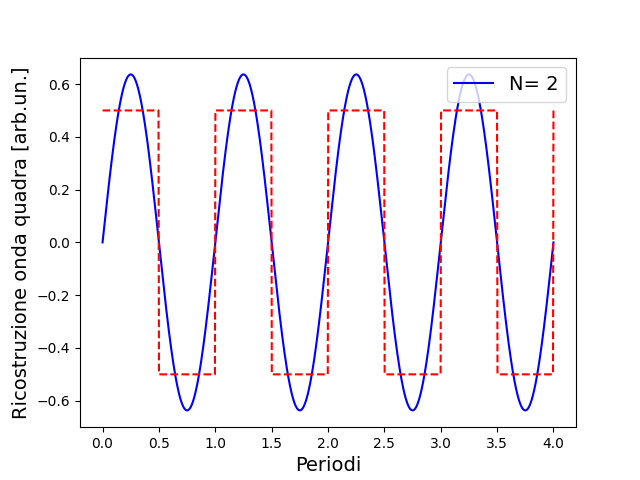
\includegraphics[width=0.49\textwidth]{img/q2.png}}
    \subfigure{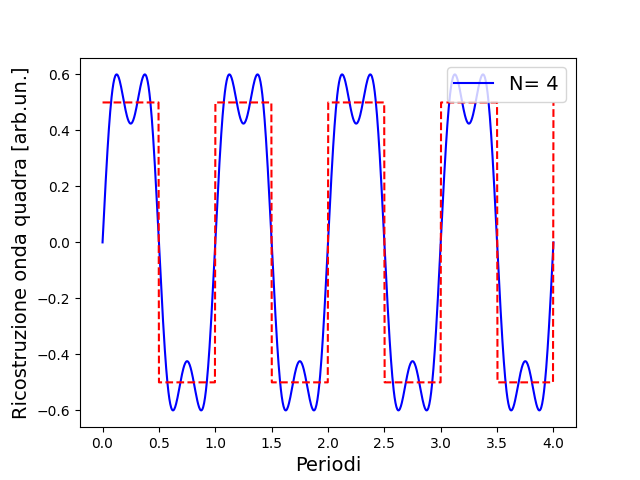
\includegraphics[width=0.49\textwidth]{img/q4.png}}
    \vspace{-0.3cm}
    \subfigure{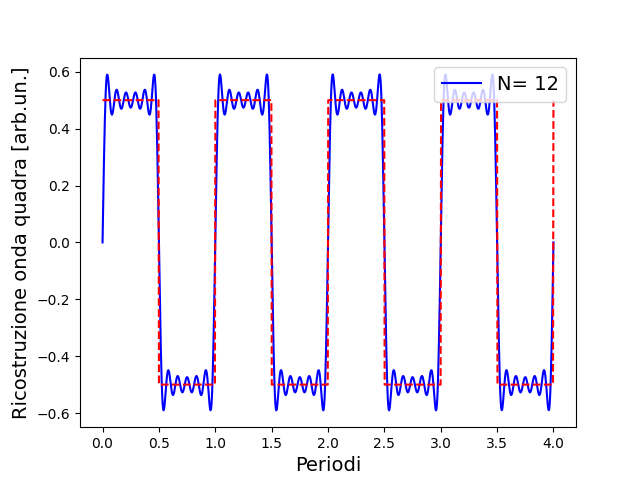
\includegraphics[width=0.49\textwidth]{img/q12.png}}
    \subfigure{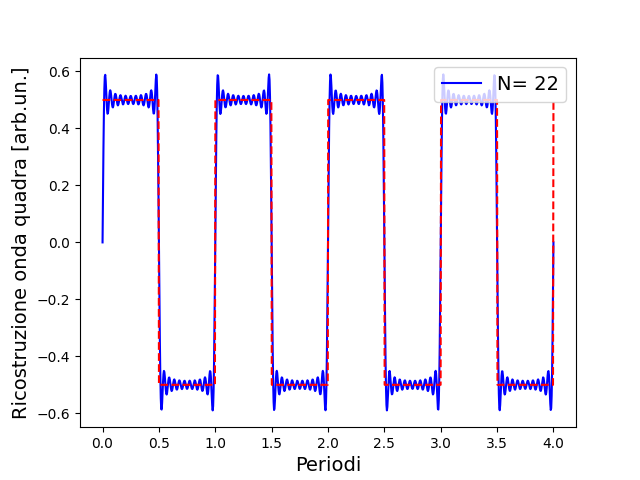
\includegraphics[width=0.49\textwidth]{img/q22.png}}
\end{figure}

\begin{figure}[H]
\vspace{-0.3cm}
    \subfigure{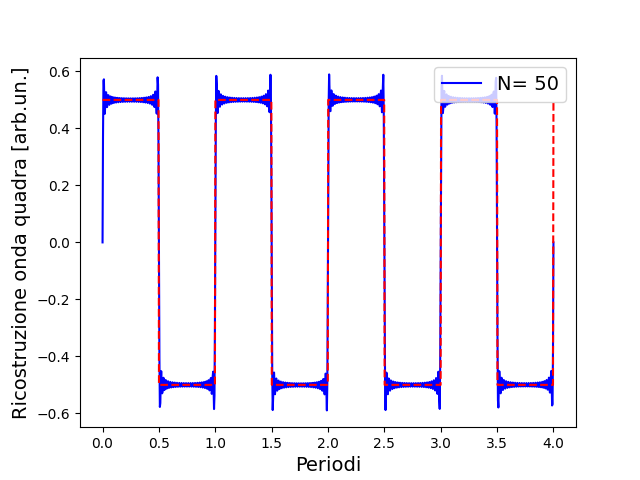
\includegraphics[width=0.49\textwidth]{img/q50.png}}
    \subfigure{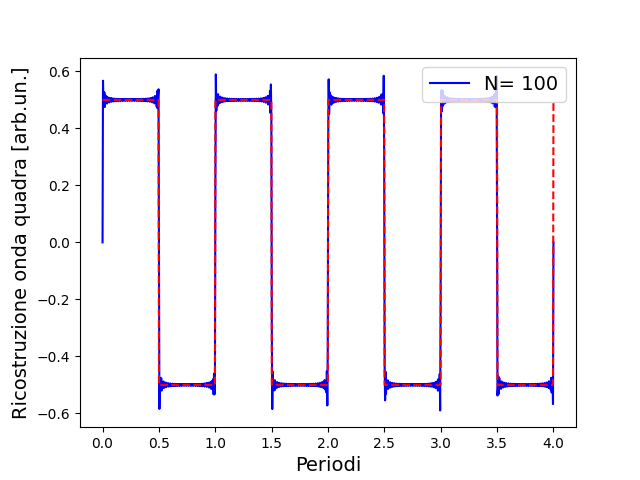
\includegraphics[width=0.49\textwidth]{img/q100.png}}
    \vspace{-0.3cm}
    \subfigure{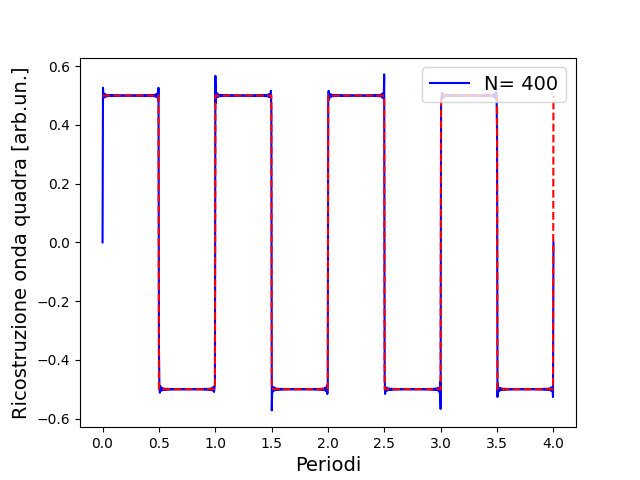
\includegraphics[width=0.49\textwidth]{img/q400.png}}
    \subfigure{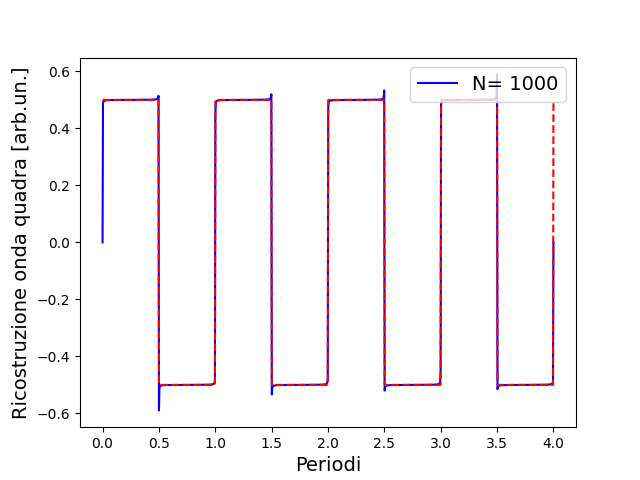
\includegraphics[width=0.49\textwidth]{img/q1000.png}}

  
    
\caption{Ricostruzione numerica di un'onda quadra mediante la serie di Fourier "Eq.\ref{eq1}",con coefficienti "Eq: \ref{eq2} e \ref{eq3}", troncata a diversi valori di \(N\) con numero di punti fisso.}  
\label{fig:imgN}  
\end{figure}  

Fissato l'array a 1000 punti, osserviamo che all'aumentare di \(N\), la ricostruzione si avvicina alla forma d'onda ideale (linea tratteggiata in rosso). Gli spikes e la loro disposizione apparentemente casuale sono dovuti alla discreta densità dei punti di campionamento.
\\\\ 


\newpage
\subsection{Forme d'onda quadre con valore di approssimazione fissato al variare dei punti.}

\begin{figure}[H]
	\vspace{-0.3cm}
    \centering
    \subfigure{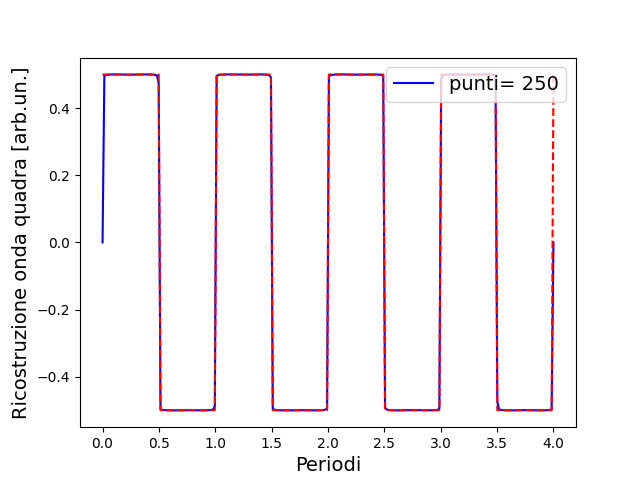
\includegraphics[width=0.49\textwidth]{img/qn250.png}}
    \subfigure{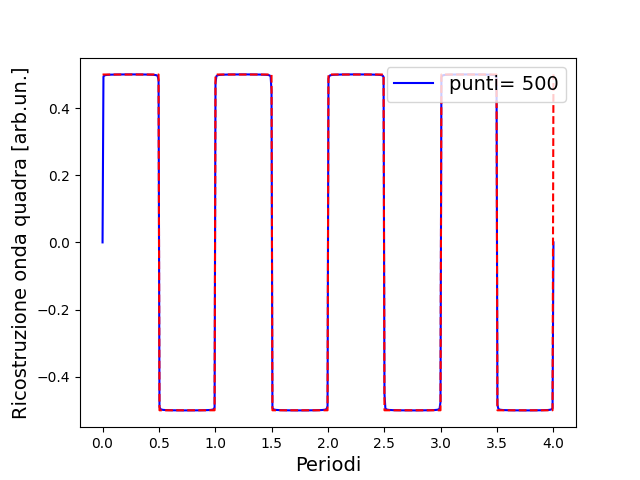
\includegraphics[width=0.49\textwidth]{img/qn500.png}}
    \vspace{-0.6cm}
\end{figure}
\begin{figure}[H]
    \subfigure{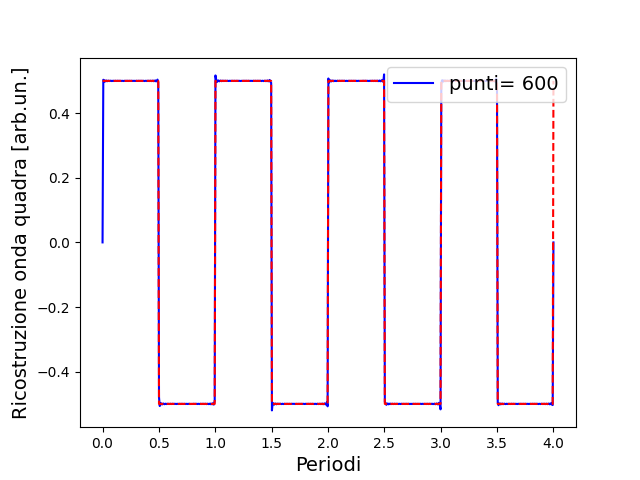
\includegraphics[width=0.49\textwidth]{img/qn600.png}}
    \subfigure{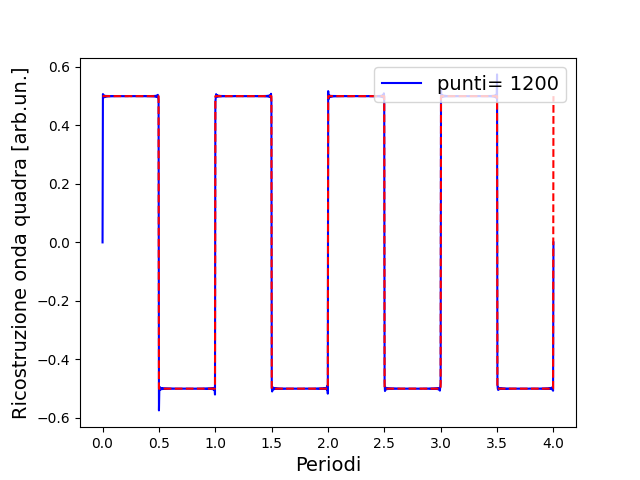
\includegraphics[width=0.49\textwidth]{img/qn1200.png}}
	\vspace{-0.3cm}
    \subfigure{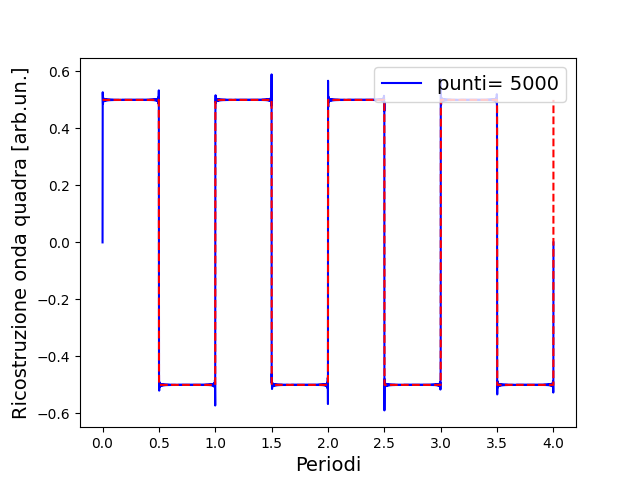
\includegraphics[width=0.49\textwidth]{img/qn5000.png}}
    \subfigure{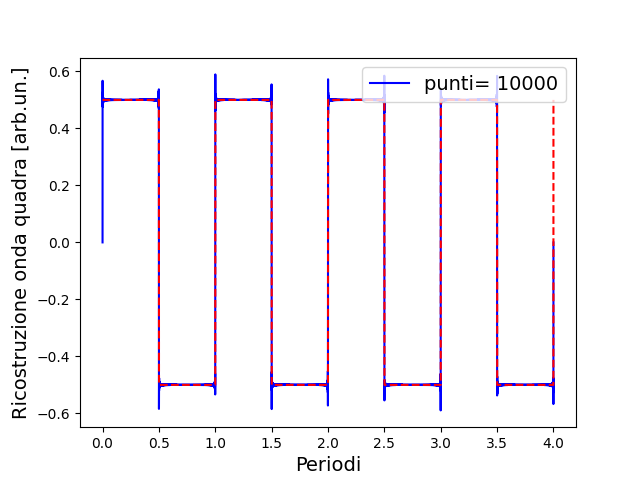
\includegraphics[width=0.49\textwidth]{img/qn10000.png}}
    
    
\caption{Ricostruzione numerica di un'onda quadra mediante la serie di Fourier "Eq.\ref{eq1}",con coefficienti "Eq: \ref{eq2} e \ref{eq3}", troncata a un valore fisso di \(N\) e con un numero variabile di punti.}  
\label{fig:imgP}  
\end{figure}  

Fissato il valore di \(N\) = 1000 , osserviamo che all'aumentare del numero di punti, la ricostruzione numerica dell'onda quadra presenta un numero sempre maggiore di  \textbf{spikes}, questo accade perché, con un maggior numero di punti, le variazioni locali della funzione vengono evidenziate in modo più dettagliato, rendendo così più visibili gli spike nelle vicinanze delle discontinuità.

\newpage
\subsection{Forme d'onda Triangolari}

I coefficienti per ricostruire le forme d'onda triangolari sono:
\begin{equation}
\label{eq4}
    b_k=(\frac{2}{k\pi})^2
\end{equation}
\begin{equation}
\label{eq5}
    c_k=0
\end{equation}
\vspace{-1cm}
\begin{figure}[H]
    \centering
    \subfigure{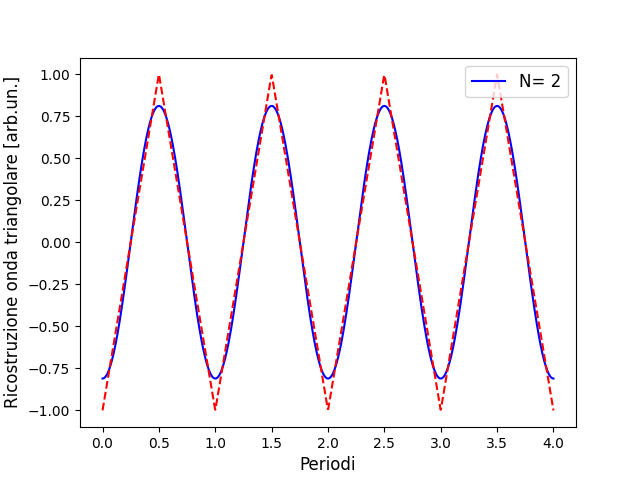
\includegraphics[width=0.49\textwidth]{img/tr2.png}}
    \subfigure{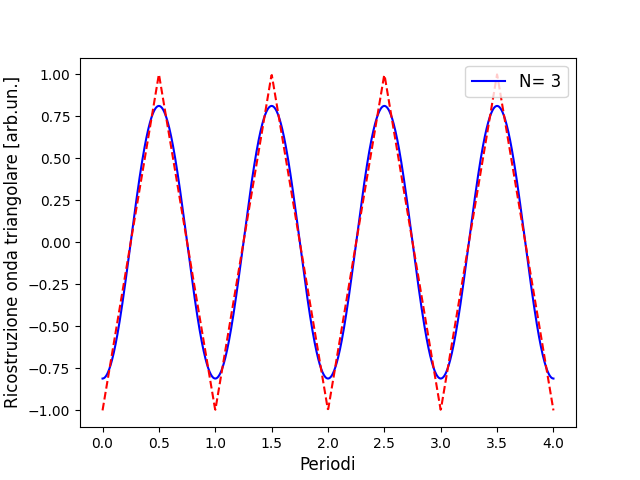
\includegraphics[width=0.49\textwidth]{img/tr3.png}}
    \vspace{-0.3cm}
    \subfigure{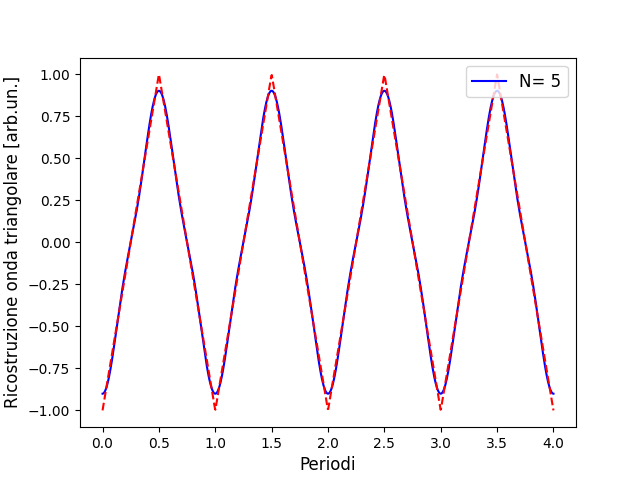
\includegraphics[width=0.49\textwidth]{img/tr5.png}}
    \subfigure{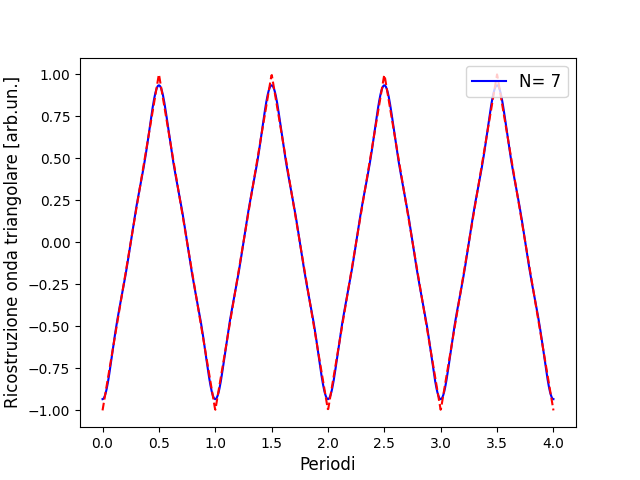
\includegraphics[width=0.49\textwidth]{img/tr7.png}}
\vspace{-0.3cm}
    \subfigure{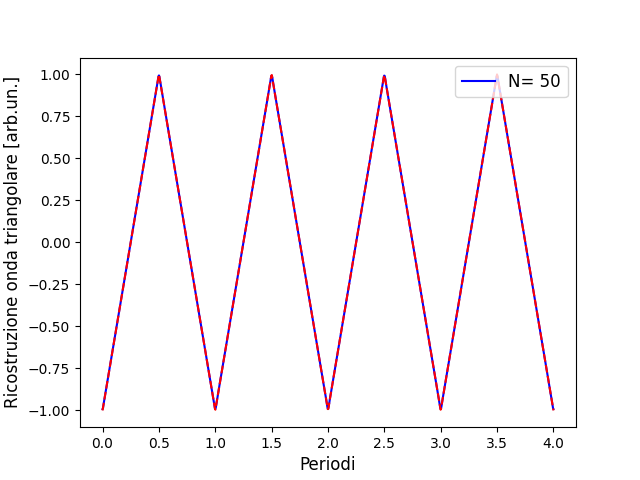
\includegraphics[width=0.49\textwidth]{img/tr50.png}}
    \subfigure{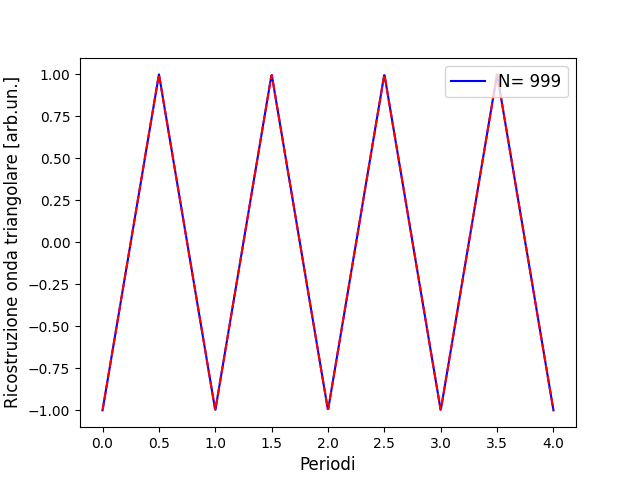
\includegraphics[width=0.49\textwidth]{img/tr999.png}}
    \vspace{-0.3cm}
    
\caption{Ricostruzione numerica di un'onda triangolare mediante la serie di Fourier "Eq.\ref{eq1}", con coefficienti in "Eq:\ref{eq4} e \ref{eq5}", troncata a diversi valori di \(N\) con numero fisso di punti.}  
\label{fig:imgTr}  
\end{figure}
Poiché la derivata dell’onda triangolare è sempre limitata,variare il numero di punti è di minore interesse, per cui concentriamoci sull'evoluzione della funzione approssimante al variare di \( N \), osservando che si adatta molto più rapidamente alla forma dell’onda triangolare. Questo avviene perché i coefficienti della serie di Fourier per l’onda triangolare diminuiscono proporzionalmente a \( \frac{1}{k^2} \), mentre quelli dell’onda quadra scalano come \( \frac{1}{k} \), rendendo la convergenza dell’onda triangolare più veloce.

\section{Comportamento degli Integratori RC: Trasformazione della Forma d’Onda Quadra}

L’analisi della risposta di un circuito integratore RC a un segnale in ingresso di tipo \textbf{onda quadra} permette di comprendere come il circuito modifichi la struttura armonica del segnale, smorzando progressivamente le alte frequenze e introducendo uno sfasamento. \\\\ Nel dominio della frequenza, un integratore RC si comporta come un \textbf{filtro passa-basso}, attenuando le componenti ad alta frequenza in base alla loro distanza dalla frequenza di taglio \( f_t \). Questo porta a una trasformazione graduale della forma d’onda in uscita, che passa da un profilo quadra a uno progressivamente più arrotondato e, per alte frequenze, approssimativamente triangolare.  

\subsection{Evoluzione della Forma d’Onda con la Frequenza}

Il comportamento dell’uscita può essere distinto in tre regimi:

\begin{itemize}
    \item \textbf{Basse frequenze (\( f \ll f_t \))}: Il circuito ha un effetto minimo sulla forma d’onda, che rimane simile all’onda quadra originale con una leggera attenuazione e sfasamento.
    \item \textbf{Frequenze prossime alla frequenza di taglio (\( f \approx f_t \))}: Le componenti alte iniziano a essere attenuate, la forma d’onda diventa più arrotondata e la transizione tra i livelli dell’onda quadra risulta smussata.
    \item \textbf{Alte frequenze (\( f \gg f_t \))}: La maggior parte delle armoniche alte è soppressa, e l’uscita assume una forma approssimativamente triangolare con una fase progressivamente ritardata.
\end{itemize}

\begin{figure}[H]
    \centering
    \vspace{-0.5cm}
    \subfigure{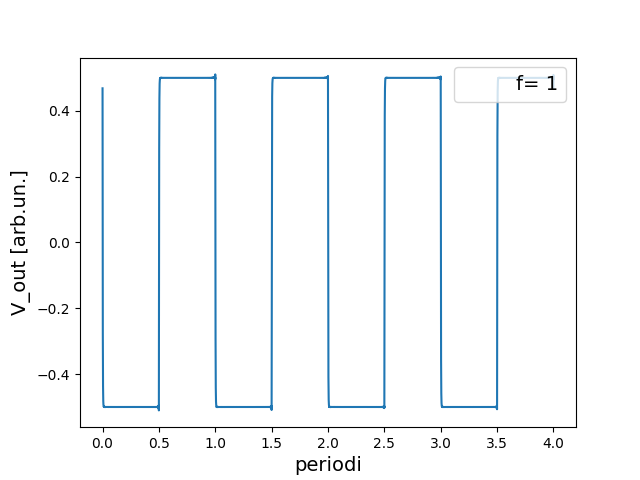
\includegraphics[width=0.49\textwidth]{img/rc1.png}}
    \subfigure{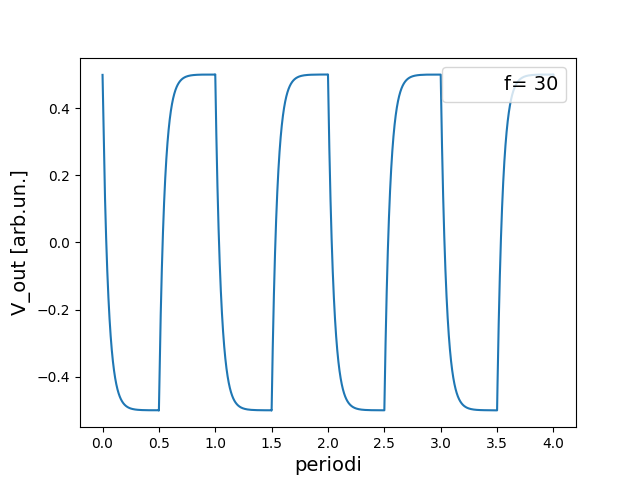
\includegraphics[width=0.49\textwidth]{img/rc30.png}}
    \vspace{-0.3cm}
    \subfigure{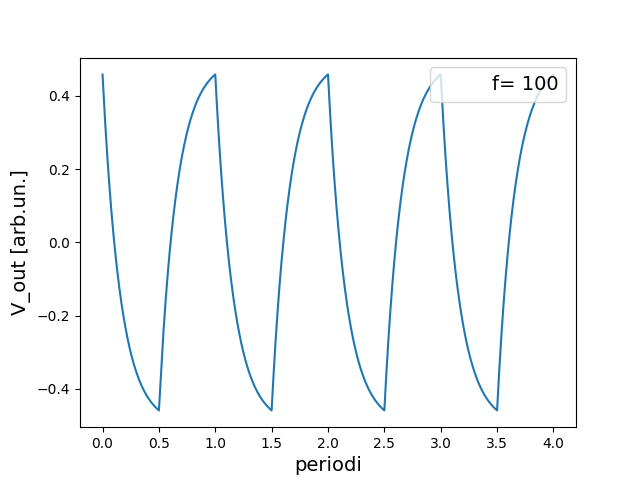
\includegraphics[width=0.49\textwidth]{img/rc100.png}}
    \subfigure{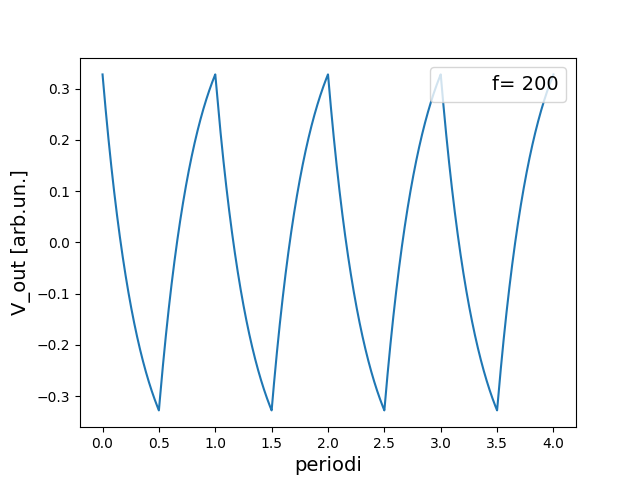
\includegraphics[width=0.49\textwidth]{img/rc200.png}}
    \end{figure}
\begin{figure}[H]
    \subfigure{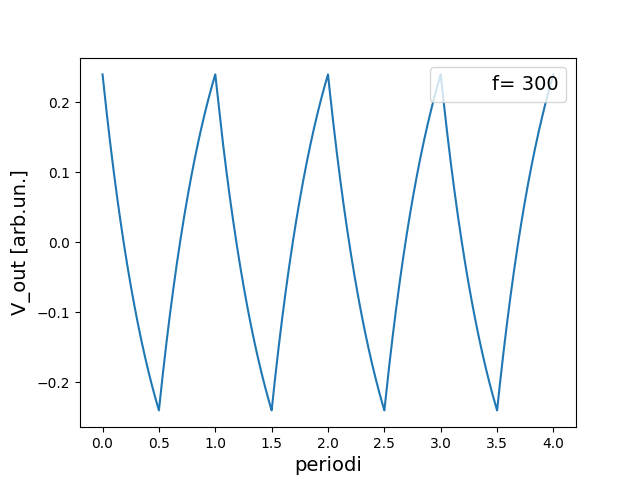
\includegraphics[width=0.49\textwidth]{img/rc300.png}}
    \subfigure{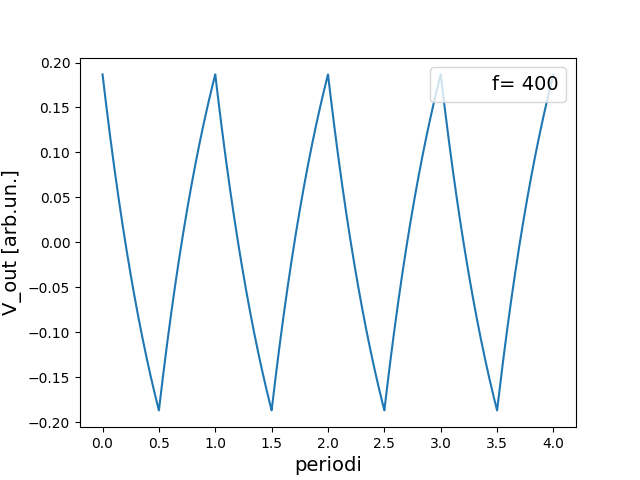
\includegraphics[width=0.49\textwidth]{img/rc400.png}}
    \vspace{-0.3cm}
    \subfigure{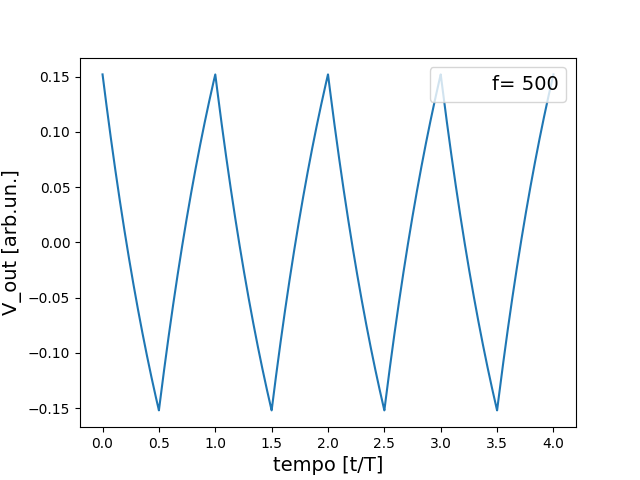
\includegraphics[width=0.49\textwidth]{img/rc500.png}}
    \subfigure{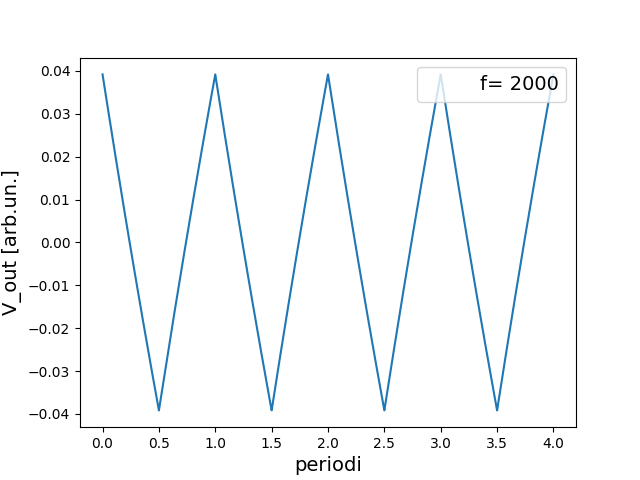
\includegraphics[width=0.49\textwidth]{img/rc2000.png}}
    
    \caption{Evoluzione della forma d’onda in uscita da un circuito integratore RC (frequenza di taglio \( f_t = 100 \, \text{Hz} \)), con segnale \textbf{quadra} in ingresso, al variare della frequenza del segnale applicato.}
    \label{fig:imgsq}
\end{figure}
Per frequenze inferiori alla frequenza di taglio, il segnale mantiene una forma simile a un’onda quadra. Con l’aumentare della frequenza, la progressiva attenuazione delle armoniche superiori porta a una forma d’onda più arrotondata, fino alla frequenza di taglio \(f_t \)=100 Hz dove c'è una netta distinzione caratterizzata da delle punte molto aguzze rispetto alle frequenze precedenti. Per frequenze elevate (\( f \gg f_t \)), l’onda in uscita assume un profilo triangolare, esattamente come previsto per la risposta del nostro circuito integratore.


\section{Fit dei dati di Arduino}

Abbiamo eseguito un fit dei dati acquisiti con Arduino utilizzando una funzione che descrive la risposta attesa di un filtro passa-basso, con l’obiettivo di confrontare il segnale sperimentale con il modello teorico e determinare i parametri ottimali. In questo fit sono stati considerati la frequenza di taglio \(f_t\), lo sfasamento \(\phi\), l'ampiezza \(A\) e l'offset \(B\). Il risultato, illustrato in Figura~\ref{fig:Fit} e riassunto in Tabella~\ref{tab:pt}, mostra una corrispondenza tra il segnale misurato e quello ricostruito.


\begin{figure}[H]
    \centering
    \vspace{-1cm}
    \includegraphics[width=0.9\textwidth]{img/fit_aj.png}
    
    \includegraphics[width=0.9\textwidth]{img/fit_cj.png}
	\caption{Simulazione numerica di un segnale a "pinna di squalo" utilizzando il modelo sviluppato precedentemente. I punti neri rappresentano i dati simulati, mentre le curve rosse indicano il best fit.}  
\label{fig:Fit}
\end{figure}
    
Nei grafici sono presenti barre d’errore, assegnate arbitrariamente con una precisione di un digit, sebbene non siano visibili. Il best fit è stato eseguito impostando \textbf{absolute sigma = false}, poiché gli errori scelti non riflettono incertezze sperimentali reali. Il valore del \(\chi^2_{\text{ridotto}}\) è pari a 1641 per il fit 1 e 941 per il fit 2, suggerendo che il secondo modello si adatta meglio ai dati simulati. Tuttavia, tale confronto è poco significativo, dato che gli errori assegnati non derivano da un processo di misura reale.

\bigskip
\begin{table}[h!]
    \centering
    \begin{tabular}{lcc}
        \hline\hline
        \textbf{Parametro} & \textbf{Fit 1} & \textbf{Fit 3} \\
        \hline
        $f$ (Hz)        & $408.55 \pm 0.09$    & $2002.44 \pm 0.97$ \\
        $f_t$ (Hz)      & $857.28 \pm 13.66$   & $182.83 \pm 9.25$ \\
        $\phi$ (rad)    & $0.030 \pm 0.007$     & $0.410 \pm 0.048$ \\
        $A$ (Digit)     & $3125.01 \pm 12.30$   & $13794.0 \pm 6912.4$ \\
        $B$ (Digit)     & $1740.88 \pm 2.55$    & $1738.04 \pm 1.93$ \\
        $\chi^2_{\text{ridotto}}$ & $1641$  & $941$ \\
        \hline\hline
    \end{tabular}
    \caption{ Nella tabella sono indicati i valori di best Fit dei parametri e il\( \chi^2_{\text{ridotto}} \)}
    \label{tab:pt}
\end{table}
\newpage

\section{Fit del guadagno onde Quadre e Sinusoidali}


Mediante la simulazione dell'uscita di un segnale da un filtro passa-basso, con onde quadre e sinusoidali come ingressi, è stata sviluppata una funzione che, prendendo in input la frequenza, restituisce in output il guadagno, ricostruendo l'onda in uscita dal filtro. L'unico parametro utilizzato è la frequenza di taglio, determinata tramite l'analisi dei dati raccolti in laboratorio.I risultati del Best fit si possono osservare in \ref{fig:FitG}.
\begin{figure}[H]
    \centering
    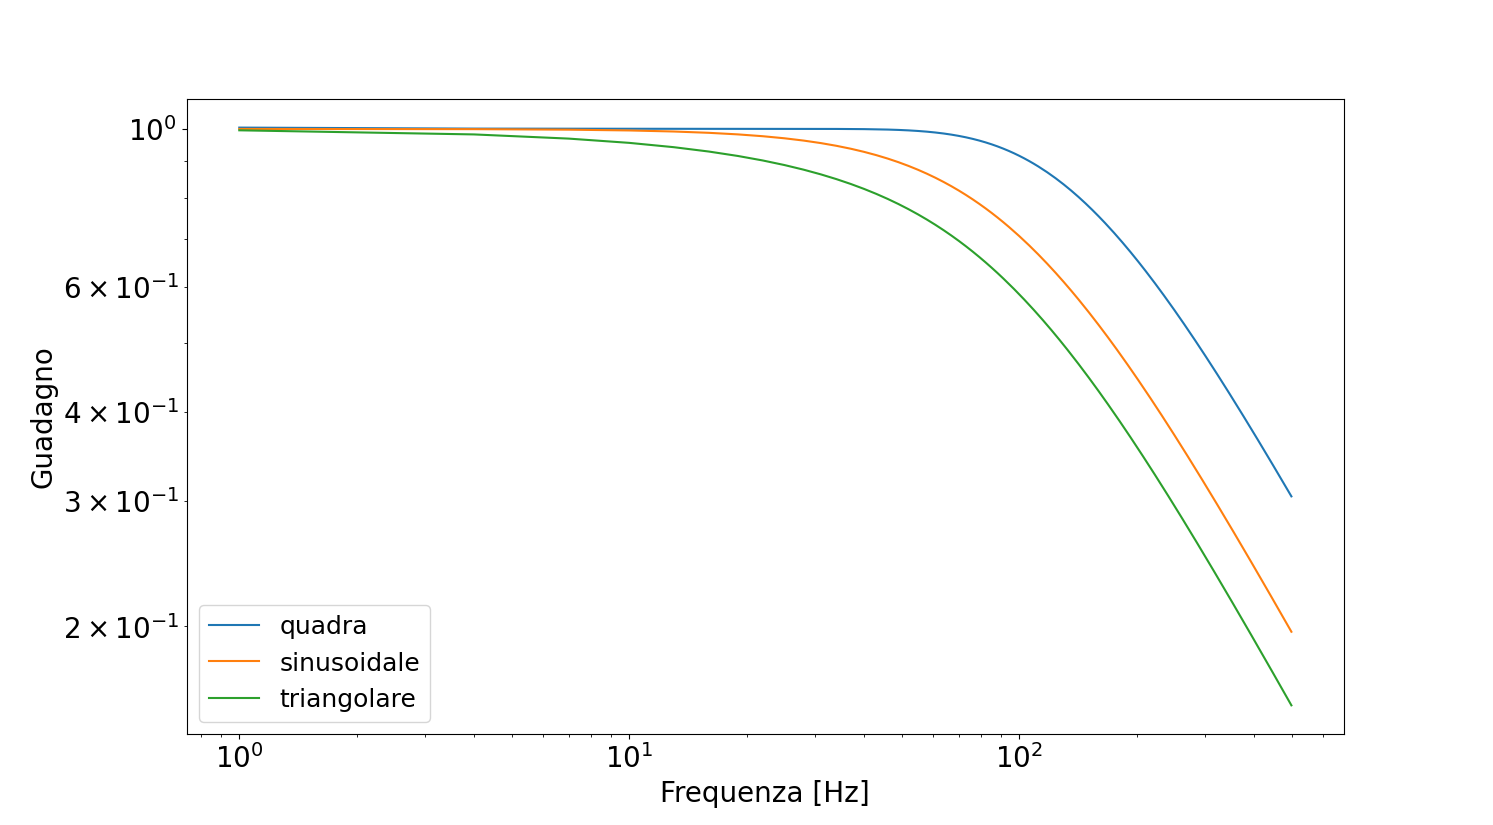
\includegraphics[width=0.9\textwidth]{img/FitG2.png}
    \caption{Simulazioni numerica dei grafici guadagno}
    \label{fig:FitG}
\end{figure}

Notiamo che i modelli delle simulazioni sono gli stessi utilizzati nel seguente Best fit:


\begin{figure}[H]
    \centering
    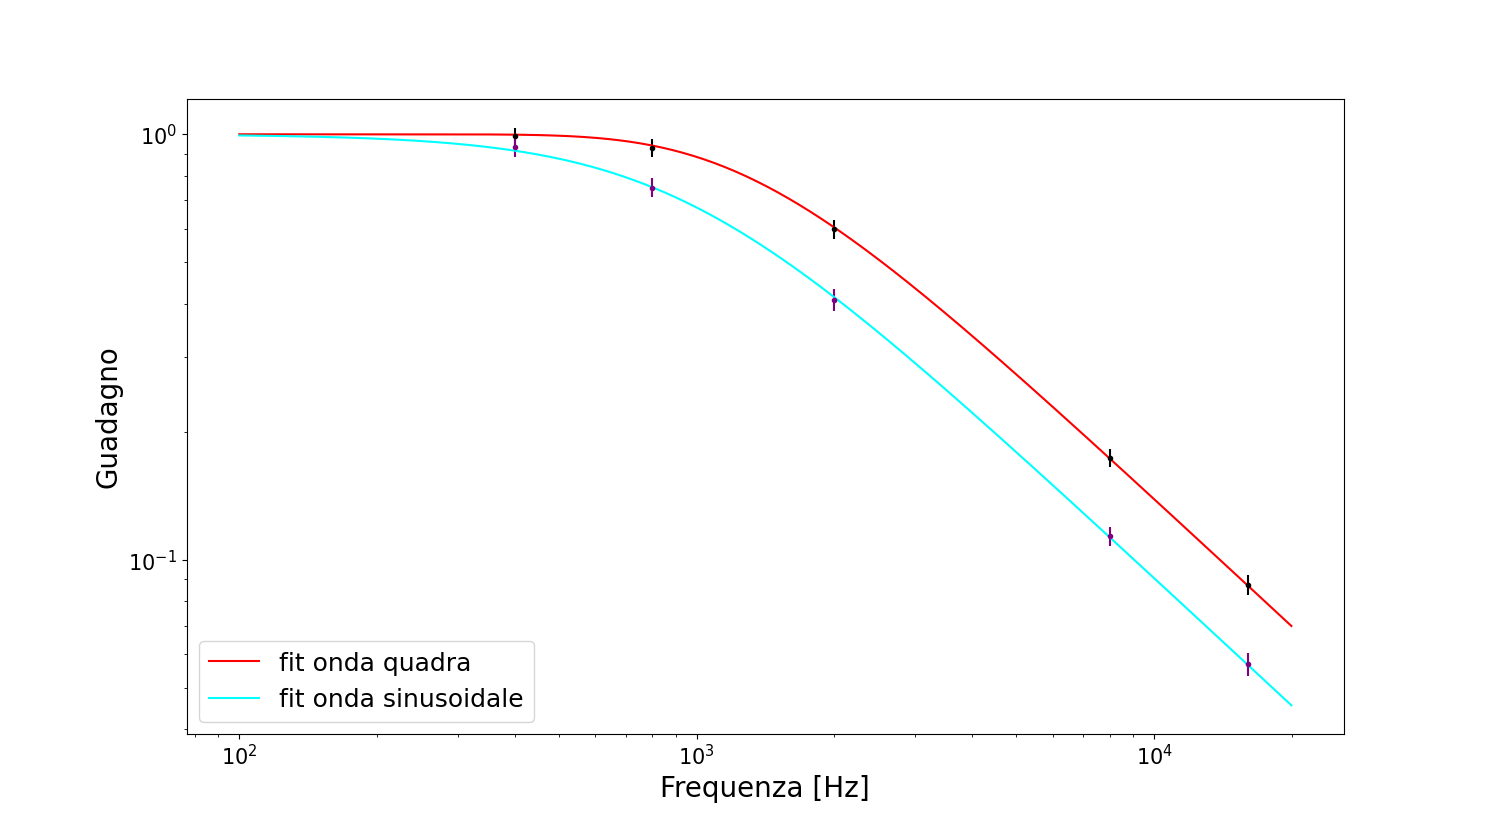
\includegraphics[width=0.9\textwidth]{img/FitG.png}
    \caption{Best fit del guadagno delle onde Quadre e Sinusoidali}
    \label{fig:FitG}
\end{figure}
\newpage
I risultati dei fit per onde quadre e sinusoidali sono riportati in Tabella \ref{tab:FitResults}.

\begin{table}[h!]
    \centering
    \begin{tabular}{lcc}
        \hline\hline
        & Quadre & Sinusoidali \\
        \hline
        $f_t$ (Hz) & $891.3 \pm 5.4$ & $909.9 \pm 6.4$ \\
        $\chi^2_{\text{ridotto}}$ & 0.142 & 0.179 \\
        \hline\hline
    \end{tabular}
    \caption{Nella tabella sono indicati i valori di best fit dei parametri e il $\chi^2_{\text{ridotto}}$. I fit sono stati effettuati con \texttt{absolute sigma=False}. Si osserva che i valori di frequenza di taglio sono compatibili tra loro, con un lieve scostamento tra onde quadre e sinusoidali.}
    \label{tab:FitResults}
\end{table}






  

\end{document}